\documentclass[runningheads]{llncs}
\usepackage{amsmath}
\usepackage{amsfonts}
\usepackage{amssymb}
\usepackage[utf8]{inputenc}
\usepackage{listings}
\usepackage{graphicx}
	    



\begin{document}
\title{Proyecto Final de Sistemas de Recuperación de Información. Motor de Búsqueda}

\author{Jessy Gigato \inst{1} \and 
Laura Tamayo\inst{2} \and 
Yasmin Cisneros\inst{3}}
\institute{Universidad de La Habana, La Habana, Cuba}
\maketitle
\begin{abstract}
	In our days, search engines have become our best allies and companions in daily use, they help us get to the information we want (in almost all cases) and resolve our most diverse concerns. These are nothing more than mechanisms that organize and distribute the information produced on the network to users who express their doubts from queries in these engines.
\end{abstract}

\section*{Introducción}


En nuestros días los motores de búsqueda se han convertido en nuestros mejores aliados y compañeros de uso cotidiano, estos nos ayudan a llegar a la información que queremos (en casi todos los casos) y resolver nuestras más diversas inquietudes. Estos no son más que mecanismos que organizan y distribuyen la información producida en la red a los usuarios que expresan sus dudas a partir de consultas en los estos motores. La recuperación de la información se ha convertido en un área sumamente importante en la Ciencia de la Computación ya que es generada diariamente una amplia cantidad de información nueva la cual presenta relevancia y su alcance debería ser importante sin obviar la información precedera.

La recuperación de información es el conjunto de actividades orientadas a facilitar la localización de determinados datos u objetos, y las interrelaciones que estos tienen a su vez con otros. Existen varias disciplinas vinculadas a esta actividad como la lingüística, la documentación o la informática. Con frecuencia, la información responde a qué es algo y que propiedades lo describe, pero tan sólo parte de la información indica cómo se elabora o se desarrolla un proceso. Este tipo de información es básicamente  conocimiento. Esta premisa muestra que el conocimiento implica dos cuestiones fundamentales: la existencia de un fin y una relación con otra información de un sistema para lograr un objetivo. En la literatura, la exposición de estas estrategias suele estar vinculada a determinado Sistema de Recuperación. Ya que el desarrollo de estas aplicaciones informáticas surgió como respuesta a la gestión de la sobreabundancia de información actual. La forma en que esta información es almacenada suele ser mediante Bases de Datos y repositorios documentales.

El trabajo presenta como objetivo principal la creación de un Motor de Búsqueda utilizando modelos de recuperación de la información el cual resulte intuitivo al usuario.


\section*{Problema Planteado}
El Proyecto Final de Sistemas de Recuperación de Información en el curso 2022 consiste en el diseño, implementación, evaluación y análisis de un Sistema de Recuperación de Información. El sistema a desarrollar debe comprender todas las etapas del proceso de recuperación de información. Es decir, desde el procesamiento de la consulta hecha por un usuario, la representación de los documentos y la consulta, el funcionamiento del motor de búsqueda y la obtención de los resultados. No hay limitaciones respecto al Modelo de Recuperación de Información que deben emplear, puede ser cualquiera de los clásicos o alguno de los alternativos, siempre atendiendo a las características de cada uno y su adecuación al escenario en el que se aplicarán.

\section*{Desarrollo}
\subsection*{Diseño del Sistema:}
En el campo de la recuperación de la información se tienen varios modelos clásicos para la recuperación de la misma. Estos serian:
\begin{itemize}
	\item Modelo Booleano
	\item Modelo Vectorial
	\item Modelo Probabilístico
\end{itemize}
Para la creación de nuestro Motor el sistema constará de la presencia de varios modelos de recuperación diferentes los cuales serán analizados de forma particular.

\subsection*{Arquitectura del Proyecto}
El Motor de Búsqueda pasara por una serie de procesos para retornarle al usuario una respuesta:
\begin{itemize}
	\item Se le entra una consulta
	\item Realiza el proceso de búsqueda en el corpus de documentos que se tiene
	\item Retorna una lista de documentos con las coincidencias y/o respuestas mas acertadas 
\end{itemize}

\subsection*{Implementación}
Cada uno de los procesos vistos anteriormente constara de una serie de pasos los cuales constituirían el pipeline (flujo) de la aplicación.\\

Parte de este pipeline sería: \\
- tokenizar la entrada \\
- limpiar dichos tokens \\
- eliminar los stopwords

\textbf{Modelo Vectorial:}\\
Primeramente mostramos un modelo vectorial (visto en conferencias), este tiene aspectos significativos como son los siguientes:

-	Este modelo es el encargado de predecir el grado de similitud del documento con respecto a la consulta relacionada.

-	Establece un umbral de similitud para la recuperación de los documentos.\\

\textbf{Representación de documentos y consulta:}\\
Este modelo de recuperación considera que cada documento esta descrito por un conjunto de palabras claves (términos indexados) los cuales presentan las siguientes características:

-	Un término indexado es una palabra que ayuda semántica mente a la captura de temas en el texto determinado.

-	Se utilizan para indexar y resumir el contenido de un documento.

-	Generalmente son sustantivos.\\


Como estamos utilizando el modelo vectorial entonces los documentos son representados mediante vectores, cuya representación es obtenida mediante la tokenización de la consulta.
\begin{equation}
	w_{ij} = frac{tf_{ij}}{\max_{k} tf_{kj}}idf_{j}
\end{equation}
Ecuación 1. Representación vista en clases\\

Donde:\\
$ w_{ij} $ - Representa el peso asociado al termino $ i $ en el documento $ j $\\
$tf_{ij}$ - Número de veces que se repite el término $i$ en el documento $j$\\
$idf_{j}$ - Frecuencia inversa del documento $j$ en la colección de documentos calculada por $\log{\frac{N}{n_j}}$\\
$n_j$ - cantidad de documentos en donde aparece el término $j$.\\

La consulta presenta la misma representación que los documentos solamente que se le aplica una formula diferente:
\begin{equation}
	(\alpha idf_i + (1-\alpha)\frac{tf_{ij}}{\max_{k} tf_{kj}}) idf_i
\end{equation}

Siendo $\alpha$ el factor de suavizado

Finalmente para realizar un ranking de los documentos se calcula la similitud entre los documentos y la consulta y son ordenados de mayor a menor y asi se devolveran.
\begin{equation}
	sim(q,d_i) = \cos(q, d_i) = \frac{q \cdot d_i}{||q|| ||d_i||}
\end{equation}

Ecuación 3. Función de similitud\\

\textbf{Ventajas y Desventajas:}\\
\textit{Ventajas:} 

-	El esquema de ponderación $tf-idf$ para los documentos mejora el rendimiento de la recuperación

-	La estrategia de coincidencia parcial permite la recuperación de documentos que se aproximen a los requerimientos de la consulta

-	La fórmula del coseno ordena los documentos de acuerdo al grado de similitud con la consulta\\

\textit{Desventajas:}

-	Asume que los términos indexados son mutuamente independientes

\subsubsection*{Modelo LSI-SVD (Indexación Semántica Latente):}
\textbf{Rentación del modelo:}
LSI es una técnica que proyecta consultas y documentos en un espacio con dimensiones semánticas “latentes”. En el espacio semántico latente, una consulta y un documento pueden tener una alta similitud de acuerdo al coseno incluso si no comparten ningún término, siempre y cuando sus términos sean semánticamente similares en un sentido que se describirá posteriormente. Podemos ver a LSI como una métrica de similitud que es una alternativa para expresar las medidas de solapamiento de palabras como $tf*idf$. El espacio semántico latente en el que proyectamos tiene menos dimensiones que el espacio original (el cual tiene tantas dimensiones como términos). LSI es, de ese modo, un método de reducción de dimensionalidad. Estas técnicas toman un conjunto de objetos que existen en un espacio de grandes-dimensiones y los representan en un espacio de pocas-dimensiones, frecuentemente en uno 2-dimensional o 3-dimensional con el propósito de visualizarlos. LSI es la aplicación de una técnica matemática particular, llamada Descomposición en Valores Singulares (SVD por sus siglas en inglés), a una matriz de términodocumento. SVD (y por lo tanto LSI) es un método de mínimos cuadrados. La proyección en el espacio semántico latente se elige de forma que las representaciones en el espacio original son reducidas tanto como sea posible cuando se mide por la suma de los cuadrados de las diferencias.\\

\textbf{Definición de la matriz Termino-Documento:}

Inicialmente se construye una matriz llamada matriz Término-Documento, $A$, para identificar las ocurrencias de los $t$ términos indexados en una colección de d documentos. En la matriz $A$, cada fila representa un término y cada columna un documento, por lo tanto, cada elemento $A_{ij}$, $1 \le i \le t, i \le j  \le d$, es el peso del término $i$ en el documento $j$. Estos pesos pueden ser calculados como el producto del peso local del término $i$ en el documento $j$, $l_{ij}$, y el peso global del término $i$ en la colección de documentos, $g_i$. Cada uno de los pesos anteriores puede ser calculado de diversas formas, en este caso utilizaremos la forma de cálculo utilizada por el modelo vectorial $(tf*idf)$\\

\textbf{SVD:}

La proyección SVD es computada por la descomposición de la matriz término-documento, $A_{txd}$ en el producto de tres matrices $T_{txn}$, $S_{nxn}$, $D_{dxn}$:
\begin{equation}
A_{txn} = T_{txn}S_{nxn}{(D_{dxn})}^T
\end{equation}

\textbf{Implicaciones de SVD para LSI:}

Podemos ver SVD como un método para la rotación de los ejes del espacio n-dimensional tal que el primer eje se ejecuta a lo largo de la dirección de la mayor variación entre los documentos, la segunda dimensión se ejecuta a lo largo de la dirección con la segunda mayor variación y así sucesivamente.

- $T$ representa los términos en este nuevo espacio. 

- $S$ representa los documentos en este nuevo espacio. 

- $D$ es una matriz diagonal que contiene los valores singulares de $A$ en orden descendente. El i-ésimo valor singular indica la variación a lo largo de la i-ésima dimensión. \\

Se puede considerar que dichas matrices ya no contienen ruido que interfiere en nuestra recuperación de información y se utilizarán para poder hacer los cálculos necesarios para obtener la similitud de los documentos con la consulta. Es posible calcular la similitud entre dos documentos, entre dos términos, entre un término y un documento, y entre una consulta y un documento mediante la manipulación de las matrices ya “limpias”. En este caso nos interesa conocer el proceso para calcular la similitud de una consulta y un documento.

\begin{figure}[htb]
\centering
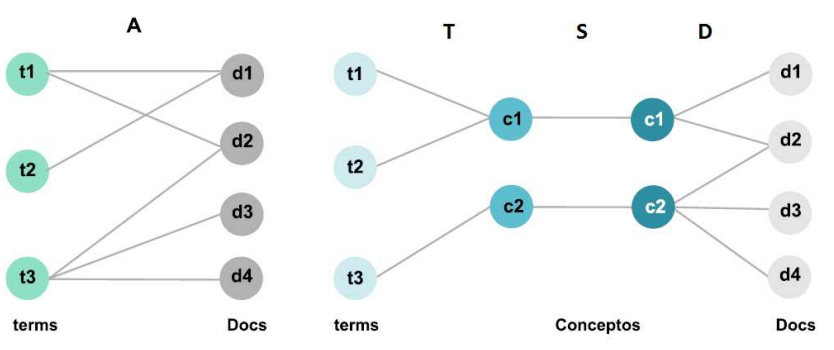
\includegraphics[width=0.8\textwidth]{grafico.png}
\caption{Representación esquemática llevada a cabo por SVD. Se puede ver que en la figura de la izquierda se conectan lo términos con sus respectivos documentos, mientras que en la derecha se observa el cómo  se tiene una capa intermedia para la reducción de dimensiones}
\label{fig:tigre}
\end{figure} 

\textbf{Representación de la consulta:}
Con el propósito de la recuperación de información, la consulta de un usuario debe ser ubicada en el espacio k-dimensional como los documentos. Como la consulta (al igual que un documento) es un conjunto de palabras, su representación en dicho espacio puede ser determinada, por ejemplo, mediante el cálculo del vector:\\
\begin{equation}
\widehat{q} = q^T T_{txn} {S^{-1}}_{nxn}
\end{equation}
Donde q es simplemente el vector de las palabras de la consulta multiplicado por los pesos apropiados. La suma de esos vectores de términos k-dimensionales se refleja por $q^T T_txn$ en la ecuación anterior, y la multiplicación por $S^{(-1)}_nxn$ diferencia los pesos de las dimensiones por separado. Por lo tanto, el vector de la consulta se obtiene de la suma ponderada de los vectores de los términos que la constituyen. El vector de la consulta puede ser comparado entonces con todos los documentos existentes y establecer un ranking por su similaridad (cercanía) a la consulta.

Un medidor común de similaridad es el coseno entre el vector de la consulta $\widehat{q}$ y el del documento (columna correspondiente en ${(D_{dxn})}^T$. Típicamente, los $z$ documentos más cercanos o todos los que excedan un umbral para el coseno serán devueltos al usuario.\\

\textbf{Ventajas y Desventajas:}\\
\textit{Ventajas:}

-	Hay coincidencia parcial. 

-	Permite hacer ranking. 

-	Al pasar al espacio de los conceptos se pueden recuperar documentos que traten sobre el mismo tema. 

-	Recupera documentos aun cuando este no contenga los términos presentes en las consultas. 

-	Permite resolver problemas de la lengua como la sinonimia y la polisemia.\\
\textit{Desventajas:}

-	Costo computacional. 

-	No se expresa la posibilidad de no tener un término, es decir, no hay posibilidades de forzar condiciones booleanas. 

-	Imposibilidad de aplicar el modelo a colecciones grandes (de decenas de millones de elementos).\\

\textbf{Rank (LTR)}

La tarea conocida como Learn to Rank consiste en dado un par consulta-documento obtener qué tan relevante es dicho documento para la consulta. Para ello representan elemento como un vector de características $x \in \Re^{n}$. El modelo es entrenado entonces para mapear ese vector de características a un valor real tal que para una consulta determinada los documentos más relevantes obtengan una puntuación más alta. \\
Como primer experimento se utilizó la biblioteca Pyterrier para el manejo del corpus utilizado(en este caso fue el vaswani) y el modelo utilizado fue el Random Forest que brinda la biblioteca sklearn.\\
El modelo usado para comparar los resultados se conoce como BM25 el cual funciona de manera similar al modelo vectorial descrito anteriormente pero la función de similaridad es la siguiente:
\begin{equation}
socre(Q,D)= \sum_{i=1}^{n}idf(q_{i}) * \frac{tf(q_{i},D)*(k_{1}+1)}{tf(q_{i},D)+k_{1}* (1-b+b*\frac{\vert D\vert}{avg(dl)})}
\end{equation}
Donde $k_{1}\in [1.2,2.0], b = 0.75$ y avg(dl) representa la longitud promedio de los documentos en la colección.\\
Las medidas que se usaron fueron el recobrado y la medida mAP. En la figura 1 se muestran los resultados obtenidos y se puede apreciar que el recobrado para 1000 documentos es mejor en el modelo con LTR mientras que el mAP es mejor en el modelo BM25.\\


\begin{figure}[htb]
\centering
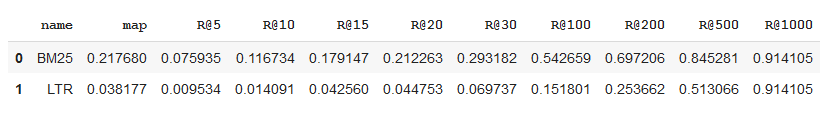
\includegraphics[width=1\textwidth]{Capture.png}
\label{fig:tigre}
\end{figure} 


\textbf{Modelo Basado en Redes Neuronales}\\
El siguiente modelo de recuperacion esta basado en Redes neuronales y su representacion es la siguiente:


\begin{figure}[htb]
\centering
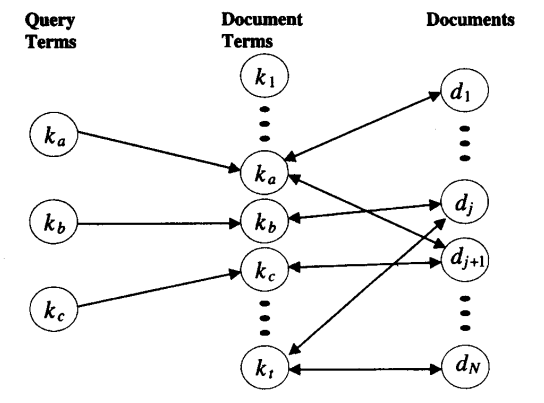
\includegraphics[width=0.8\textwidth]{red.png}
\caption{Representación de la red neuronal de recuperación de la informacional}
\label{fig:tigre}
\end{figure} 

Esta red neuronal consta de 3 capas:

-	La primera es la capa representativa de la consulta que contiene los términos indexados pertenecientes a la misma.

-	La segunta es representadas por todos los términos  pertenecientes al SRI.

-	La tercera contiene la serie de documentos \\


\textbf{Expansión de Consulta}

La expansión de consulta consiste en seleccionar y agregar términos a la consulta del usuario con el objetivo de minimizar la falta de coincidencia entre la consulta y el documento y, por lo tanto, mejorar el rendimiento de la recuperación.

En este caso la expansión de consulta se realizo mediante la seleccion de sinónimos (Que tiene el mismo significado que otra u otras palabras), holonimos y meronimos (ambas relacionado con respecto a partes, ejemplo de animal: patas).

\subsection*{Herramientas utilizadas en el sistema}

Las herramientas computacionales que fueron utilizadas para la implementación del proyecto son:\\

Las bibliotecas de Python:

-	sklearn: Uso del modelo vectorial.

-	nltk: para el procesamiento del corpus, eliminación de stop words y expansión de consulta.

-	keras: Modelo utilizando redes neuronales.

-	PyQt5: Encargado de la interfaz visual de la aplicación.


\section*{Conclusiones}
(Trabajando)

\section*{Referencias}
\begin{enumerate}
\item Documentacion de pyterrier.
\item Conferencias de 5to año Sistema de Recuperación de la Información.
\end{enumerate} 


\end{document}